\section{Answer changes and selective accuracy}
\label{sec:metrics}

The matched same-span control gives the response to rewriting an event while
preserving its class. To interpret the contrast with a different-class edit,
let $C_o$, $C_d$, and $C_s$ denote binary correctness on the original,
different-class, and same-class inputs, with $a_j=\mathbb{E}[C_j]$. For valid
binary answers with fixed option-to-class mappings, the original and
same-class inputs share a truth label. The different-class input has the other
label. Their answer-change probabilities satisfy
\begin{equation}
\begin{aligned}
A_s &= \mathbb{E}[C_o+C_s-2C_oC_s],\\
A_d &= \mathbb{E}[1-C_o-C_d+2C_oC_d].
\end{aligned}
\label{eq:binary-change}
\end{equation}
The answer-change gap $\Delta=A_d-A_s$ combines marginal correctness and
dependence between condition outcomes. Factoring the correctness products
gives the reference value under independence of original correctness from each
edited outcome,
\begin{equation}
G_{\mathrm{ind}}=(2a_o-1)(a_d+a_s-1).
\label{eq:independent-reference}
\end{equation}
The exact relationship is
\begin{equation}
\Delta=G_{\mathrm{ind}}+2\operatorname{Cov}(C_o,C_d)
  +2\operatorname{Cov}(C_o,C_s).
\label{eq:dependence-correction}
\end{equation}
The reference assumes independence of original correctness from each edited
outcome, without requiring independence between the edited outcomes. It is an
algebraic benchmark based on marginal accuracies. Equation~\ref{eq:dependence-correction}
shows that the difference between the observed gap and this reference equals
the covariance correction. Figure~\ref{fig:class} relates original accuracy
to the gap for each evaluated query class and model.

\begin{figure}[t]
\centering
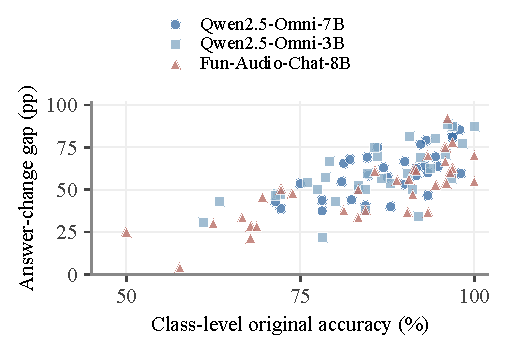
\includegraphics[width=\columnwidth]{figures/reference_class.pdf}
\caption{Class-level original accuracy versus the different-class minus
same-class answer-change gap. Each point represents one of 33 query classes
for one model. Both quantities use the same evaluation trials.}
\label{fig:class}
\end{figure}

Selective accuracy measures whether a revised answer identifies the inserted
class on eligible trials. An eligible trial has correct answers on both the
original and same-class inputs. Each soundscape $i$ contributes two option-order
trials $\mathcal T_i$. Define the eligible trials $\mathcal C$ and soundscapes
$\mathcal I_{\mathcal C}$ containing at least one eligible trial. The reported
selective accuracy is
\begin{equation}
\begin{aligned}
\mathcal C &= \{t\mid C_o(t)=C_s(t)=1\},\\
\mathcal I_{\mathcal C} &= \{i\mid \mathcal T_i\cap\mathcal C\ne\varnothing\},\\
F_{\mathcal C} &= \frac{1}{|\mathcal I_{\mathcal C}|}
\sum_{i\in\mathcal I_{\mathcal C}}
\frac{\sum_{t\in\mathcal T_i\cap\mathcal C}C_d(t)}
{|\mathcal T_i\cap\mathcal C|}.
\end{aligned}
\label{eq:selective-accuracy}
\end{equation}
On an eligible trial, identifying the different-class donor also means
changing the original answer in the correct direction. Eligible trials are
averaged within each soundscape before eligible soundscapes receive equal
weight. Eligibility depends on each model's responses, so a soundscape may
contribute one option order. Table~\ref{tab:follow} reports eligible-trial and
eligible-soundscape counts as coverage.
